% paper proposal for the Modelica 2017 Conference

%%% By default the modelica LaTeX class uses bibtex and natbib for refrences
\documentclass{resources/modelica}
%%% As alternative also for unicode and @online support
%%% use the more modern biber and biblatex instead
%\documentclass[backend=biber]{modelica}
%\addbibresource{example-paper.bib}
%\usepackage[utf8]{luainputenc} % utf8 input encoding that should work for both pdflatex and lualatex, but might not be available in every installation
\usepackage[utf8]{inputenc} % utf8 input encoding which should work with pdflatex, but not lualatex
\usepackage{cleveref}
\usepackage{caption} % subfloats (http://en.wikibooks.org/wiki/LaTeX/Floats,_Figures_and_Captions#Subfloats)
\usepackage{subcaption} % subfloats (http://en.wikibooks.org/wiki/LaTeX/Floats,_Figures_and_Captions#Subfloats)

\hypersetup{%
	pdftitle  = {Towards a Standard-Conform, Platform-Generic and Feature-Rich Modelica Device Drivers Library},
	pdfauthor = {Bernhard Thiele, Thomas Beutlich, Volker Waurich, Martin Sjölund,
	Tobias Bellmann}, pdfsubject = {12th International Modelica Conference 2017},
  pdfkeywords = {Modelica, embedded systems, real-time simulation},
	colorlinks,
	linkcolor=black,
	urlcolor=black,
	citecolor=black,
	pdfpagelayout = SinglePage,
	pdfcreator = pdflatex,
	pdfproducer = pdflatex}

\lstset{language = c,
       % basicstyle=\fontsize{9pt}{10.5pt}\selectfont,
       basicstyle=\fontsize{9pt}{10.5pt}\ttfamily,
       backgroundcolor = \color{white}}
\newcommand{\clang}[1]{\lstinline[language=c]|#1|}

\newcommand{\modelica}[1]{\lstinline[language=modelica]|#1|}
\newcommand{\BTHI}[1]{{\color{blue}{$\parallel_\textrm{BTHI}$#1$\parallel$}}}
\newcommand{\TBEU}[1]{{\color{orange}{$\parallel_\textrm{TBEU}$#1$\parallel$}}}
\newcommand{\VWAU}[1]{{\color{red}{$\parallel_\textrm{VWAU}$#1$\parallel$}}}
\newcommand{\MSJO}[1]{{\color{green}{$\parallel_\textrm{MSJO}$#1$\parallel$}}}
\newcommand{\TBEL}[1]{{\color{magenta}{$\parallel_\textrm{TBEL}$#1$\parallel$}}}

\crefformat{footnote}{#2\footnotemark[#1]#3}

% begin the document
\begin{document}
\thispagestyle{empty}

\title{Towards a Standard-Conform, Platform-Generic and Feature-Rich Modelica Device Drivers Library}
\author[1]{Bernhard Thiele}
\author[2]{Thomas Beutlich}
\author[3]{Volker Waurich}
\author[1]{Martin Sjölund}
\author[4]{Tobias Bellmann}
\affil[1]{PELAB, Linköping University, Sweden, {\small\texttt{\{bernhard.thiele,martin.sjoelund\}@liu.se}}}
\affil[2]{ESI ITI GmbH, Germany, {\small\texttt{thomas.beutlich@esi-group.com}}}
\affil[3]{Chair of Construction Machinery, TU Dresden, Germany, {\small\texttt{volker.waurich@tu-dresden.de}}}
\affil[4]{Institute of System Dynamics and Control, DLR, Germany, {\small\texttt{tobias.bellmann@dlr.de}}}

\date{} % <--- leave date empty
\maketitle\thispagestyle{empty} %% <-- you need this for the first page
\abstract{%
There are many cases where simulation applications need to interact with their
environment. Typical examples are Human-in-the-Loop (HITL) simulators (including
flight, driving, and marine training simulators), Hardware-in-the-Loop (HIL)
simulators, but also offline process simulators which cannot operate in a
completely self-contained manner and therefore need to be coupled to external
applications. Embedded control applications are another related area which
requires that applications interact with their environment. The
\emph{Modelica\_DeviceDrivers} library, which had its first release as
open-source library in 2012, tries to cater for such use cases. This paper
describes the library for the first time and reports about the numerous
challenges that the project experienced to meet its goal of supporting several
platforms and tools within a standard-conform, platform-generic, feature-rich,
and easy-to-use Modelica library.}

\noindent\emph{Keywords: HITL, HIL, real-time, embedded control applications,
external C}

\section{Introduction}
\BTHI{Bernhard, Tobias}\\

The most common usage of Modelica models is for offline simulation experiments.
However, in many cases simulations need to interact with their environment or
other software components.
Typical examples are Human-in-the-Loop (HITL) simulators (including flight,
driving, and marine training simulators), Hardware-in-the-Loop (HIL) simulators,
but also offline process simulators which cannot operate in a completely
self-contained manner and therefore need to be coupled to external applications.
Furthermore, Modelica can be used for developing (model-based) control
applications which also require interaction with their environment.

There are different approaches for enabling the above mentioned applications in
the context of Modelica. Several development environments offer tool chains for
real-time simulation and/or model-based development of embedded control
applications.
Some of these environments can be coupled with Modelica tools, by wrapping code
which is generated from Modelica tools into respective third-party tool-internal
representations which can be connected to hardware devices in the respective
development environment (\textit{e.g.}, Dymola\footnote{Dassault Systèmes,
\url{https://www.3ds.com}} via its DymolaBlock interface to the
MATLAB/Simulink\footnote{\label{tmw}The MathWorks, \url{https://mathworks.com}}
tool chain, OpenModelica\footnote{Open Source Modelica Consortium (OSMC),
\url{https://www.openmodelica.org}} via customized tool chains
\citep{Worschech2012}, SimulationX\footnote{SimulationX by ESI,
\url{https://www.simulationx.com}} via Code Export for Simulink/Simulink
Coder\cref{tmw} or HIL environments like dSPACE
DS1006\footnote{\label{dspace}dSPACE, \url{https://www.dspace.com}}, NI
VeriStand\footnote{National Instruments, \url{http://www.ni.com}} or ETAS
LABCAR\footnote{ETAS, \url{http://www.etas.com}} \citep{Blochwitz2009}).
Sometimes it may also be possible for a Modelica tool to generate Functional
Mock-up Units (FMUs) which can be imported into compatible development
environments, like the tool chain provided for the SCALEXIO\cref{dspace}
platform.

The \emph{Modelica\_DeviceDrivers} (MDD) library uses a different approach.
The MDD library provides access to external devices by utilizing Modelica's external
function interface for interfacing to the C API of various device drivers directly from Modelica
models (see Section~\ref{ModelicaDeviceDrivers}).

Historically, the origins of the MDD library can be traced back to the
\emph{ExternalDevices} library \citep{Bellmann2009}, an internal
DLR\footnote{Deutsches Zentrum für Luft- und Raumfahrt (DLR), German Aerospace
Center, \url{http://www.dlr.de}} Modelica library developed for the interactive
simulation and visualization of Modelica models. The \emph{ExternalDevices}
library already supported UDP and shared memory communication
as well as several input devices (keyboard, 3Dconnexion
SpaceMouse\footnote{3Dconnexion, \url{https://www.3dconnexion.com}}, and game
controller). Additionally, it featured a model-integrated real-time
visualization system, the foundation of the later \emph{DLR Visualization} library \citep{Hellerer2014}.

However, the \emph{ExternalDevices} library was limited to
Microsoft Windows and was developed to be used only with
the Dymola tool. In the further course of development it was decided to
split the \emph{ExternalDevices} library into the commercial DLR
Visualization library and an open-source cross-platform hardware interface
library, the \emph{Modelica\_DeviceDrivers} library.


% \BTHI{TODO: Bernhard, Tobias , \cite{Elmqvist2009}}


\section{Modelica\_DeviceDrivers}
\label{ModelicaDeviceDrivers}
\BTHI{TODO: Bernhard, Thomas, Volker}

The MDD library allows to access hardware devices from Modelica models.
This is achieved by using the Modelica external C interface to call the
appropriate C driver functions provided by the underlying operating system (see
Section~\ref{sec:CrossPlatformSupport}).

The library is organized in several layers as indicated in
Figure~\ref{fig:MDDLayeredArchitecture}. It
provides two high-level Drag \& Drop block interfaces. The first (\texttt{Blocks}) is
compatible to Modelica 3.2, using the traditional \modelica{when sample()}
element for periodically calling Modelica functions from the \textsf{Function Layer}. The second
(\texttt{ClockedBlocks}) uses the synchronous language elements extension
introduced in Modelica 3.3 and is compatible with the
\emph{Modelica\_Synchronous} library \citep{Otter2012}. Due to this support, the
MDD library formally depends on the \emph{Modelica\_Synchronous} library, but in
practice the \emph{Modelica\_Synchronous} library (and tool support for the
synchronous language elements extension) is only required if one actually wants
to use the clocked block interface.
\begin{figure}[htb]
\begin{center}
  \includegraphics[width=\columnwidth]{figures/MDDLayeredArchitecture}
  \caption{MDD layered architecture.}
  \label{fig:MDDLayeredArchitecture}
\end{center}
\end{figure}

\subsection{Cross-Platform Support}
\label{sec:CrossPlatformSupport}

As of MDD v1.5.0, Microsoft Windows and Linux are supported as main platforms,
but prototypical work also targets popular embedded systems boards directly (see
Section~\ref{sec:EmbeddedControl}).

When accessing hardware devices, a Modelica model or
application calls Modelica functions from the \textsf{Function Layer} (see
Figure~\ref{fig:MDDLayeredArchitecture}). These Modelica functions provide a
generic interface to the underlying \textsf{C-Code Layer} which is accessed by
Modelica's external function interface.
The platform differentiation is handled in the \textsf{C-Code Layer} which
uses preprocessor directives for conditional inclusion/exclusion of
platform-specific code (\mbox{\clang{#if}}, \mbox{\clang{#else}},
\mbox{\clang{#endif}}, etc.) similarly to the code fragment below.
\begin{lstlisting}[language=C]
#if defined(_MSC_VER) || defined(__CYGWIN__) || defined(__MINGW32__)
#include <windows.h>
/* Microsoft Windows specific code goes here */
#elif defined(__linux__)
#include <unistd.h>
/* Linux specific code goes here */
#else
#error "Modelica_DeviceDrivers: Unsupported compiler or platform"
#endif
\end{lstlisting}

\subsection{Extended Tool Support}
\label{sec:ExtendedToolSupport}

Back in 2009, the library was developed using the Dymola tool. With MDD v1.4.0,
considerable development efforts have been spent on the Modelica compliance of
the library in order to better support SimulationX and OpenModelica.

Since OpenModelica 1.11 Beta 1 the MDD Communication blocks are finally
supported by OpenModelica. For achieving this, it was necessary to change parts
of the library (under the constraint of maintaining backwards compatibility),
and at the same time, to extend the abilities of respective tools (partly by
providing support for constructs which are not (yet) allowed by the Modelica
language standard). This is discussed in more detail in
Section~\ref{sec:ModelicaStandardCompliance}.


\subsection{Library Structure}
\label{sec:LibraryStructure}

Figure~\ref{fig:MDDPackageBrowseScreenshot} shows a screenshot of the package
browser view with loaded MDD library. The first two sub packages
\modelica{Blocks} and \modelica{ClockedBlocks} provide the drag \& drop blocks
which correspond to the \textsf{Block Layer} of
Figure~\ref{fig:MDDLayeredArchitecture}. The remaining sub packages (except
\modelica{Utilities} and \modelica{EmbeddedTargets}) provide the
\textsf{Function Layer}.
Both layers use sub packages for subdividing the provided functionality into
different groups. Package \modelica{EmbeddedTargets} contains highly
target specific function and blocks for supporting restricted
embedded systems like the Arduino microcontroller (see
Section~\ref{sec:Applications}).

\begin{figure}[htb]
  \centering
  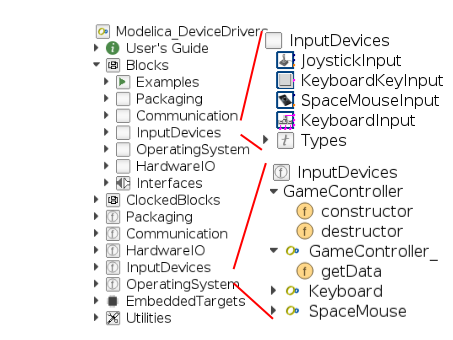
\includegraphics[width=\columnwidth]{figures/MDDPackageBrowseScreenshot}
  \caption{MDD library structure.}
  \label{fig:MDDPackageBrowseScreenshot}
\end{figure}

Furthermore, Figure~\ref{fig:MDDPackageBrowseScreenshot} gives an indication
about the relation between the block layer and the function layer. Typically, a
device driver block will instantiate a corresponding external object from the
function layer. Modelica's external objects allow to maintain internal memory
between calls to external functions. This allows to open and initialize hardware
devices once, during Modelica's initialization phase, and maintain the so
created device handlers in memory for accessing them in subsequent simulation phases.
For example, the \modelica{JoystickInput} block creates an instance of the
external object class \mbox{\modelica{GameController}.} The package
\modelica{GameController_} collects functions that can operate on external
objects of type \modelica{GameController}. The package provides the function
\modelica{getData(..)}, which takes a \modelica{GameController} object as
argument and returns the values of the axes and buttons of its associated
hardware device.

A good way of learning how to use the block layer interface of the library is by
exploring the \modelica{Examples} package. Care has been taken to provide
self-explanatory usage examples for the provided device driver blocks.

\subsection{Interfaces}

MDD library functionality can be accessed by drag \& drop of blocks
from the \modelica{Blocks} and \modelica{ClockedBlocks} sub packages, or by
direct calls to the underlying functions.

An example, which directly uses the function layer for accessing a
game controller is given below:
\begin{lstlisting}[language=modelica]
model GameControllerExample
  import
    Modelica_DeviceDrivers.InputDevices.*;
  parameter Integer id = 0 "0 = first attached game controller";
  GameController gc = GameController(id);
  Real axesRaw[6];
  Integer buttons[32], pOV;
equation
  when sample(0,0.1) then
    (axesRaw,buttons,pOV) = GameController_.getData(gc);
  end when;
end GameControllerExample;
\end{lstlisting}

The code above creates an external object named \mbox{\modelica{gc}.} The
constructor for this object takes the argument \mbox{\modelica{id}.} This
argument allows to specify which controller to use if several game controllers are attached to the
system. The function \modelica{getData} is called periodically within a
\modelica{when}-clause. It takes the external object \modelica{gc} as
argument and returns vectors which contain the values read from the
associated game controller. The vector is pre-dimensioned, so that it can attune
to controllers featuring as much as six axes, 32 buttons and a POV (point of
view) switch. The actually provided data depends on the game
controller hardware. Tests with the actual hardware are needed for determining
which vector entry corresponds to which physical axis or button.

Figure~\ref{fig:JoystickBlocks} shows how game controllers can be accessed by
simply dragging \& dropping a \modelica{JoystickInput} block into the diagram
view of a Modelica tool. While Figure~\ref{fig:MDDJoystick} uses the block found
below the \modelica{Blocks} package,
Figure~\ref{fig:MDDJoystickClocked} uses the corresponding clocked variant from
\modelica{ClockedBlocks}. The additional blocks \modelica{periodicClock} and
\modelica{assignClock} are from the \emph{Modelica\_Synchronous} library. They
associate a periodic clock to the variables and equations within the
\modelica{JoystickInput} block. As a result, the underlying
\modelica{GameController_.getData(..)} function will be called whenever the
associated clock ticks (\textit{i.e.}, every $0.1\,\mathrm{s}$ in the presented
example).

\begin{figure}[htb]
  \centering
  \begin{subfigure}[b]{0.45\columnwidth}
     \centering
     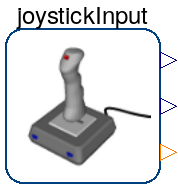
\includegraphics[width=0.55\textwidth]{figures/MDDJoystick}
     \caption{Using \modelica{Blocks}}
     \label{fig:MDDJoystick}
  \end{subfigure}%
  ~ %add desired spacing between images, e. g. ~, \quad, \qquad, \hfill etc.
    %(or a blank line to force the subfigure onto a new line)
  \begin{subfigure}[b]{0.45\columnwidth}
          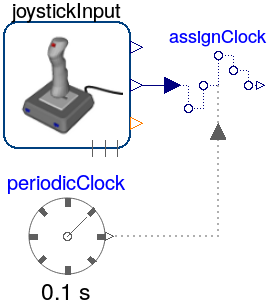
\includegraphics[width=\textwidth]{figures/MDDJoystickClocked}
          \caption{Using \modelica{ClockedBlocks}}
          \label{fig:MDDJoystickClocked}
  \end{subfigure}
  \caption{Accessing game controller devices by using the
  \modelica{JoystickInput} block from the \modelica{Blocks}, or the
  \modelica{ClockedBlocks} package.}
  \label{fig:JoystickBlocks}
\end{figure}

The example models can be simulated, but real-time synchronization is
required for allowing enough time to pass, so that user inputs can be
recognized.
The MDD library provides convenient support for (soft) real-time
synchronization\footnote{See documentation to block
\mbox{\modelica{SynchronizeRealtime}.}
%\url{https://build.openmodelica.org/Documentation/Modelica_DeviceDrivers.Blocks.OperatingSystem.SynchronizeRealtime.html}
}.
However, a user should consider that Modelica tools may provide better (tool-specific) mechanisms for real-time synchronization.

\subsection{Features}

The MDD library has grown to support a respectable amount of hardware devices
and associated features which will be briefly presented in this section.

\subsubsection{Input Devices}

\begin{figure}[htb]
  \centering
  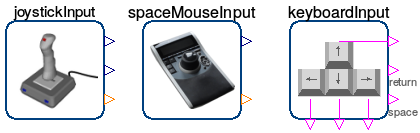
\includegraphics[width=0.7\columnwidth]{figures/OverviewInputDevices}
  \caption{Supported input devices from the \modelica{Blocks} package.}
  \label{fig:OverviewInputDevices}
\end{figure}

Standard input devices like keyboard and game controllers are ubiquitously
available on the market and allow to quickly build up interactive simulations.
MDD provides blocks for using the generic keyboard and game controller interface
of Windows or Linux (see Figure~\ref{fig:OverviewInputDevices}). Also more
specialized hardware like the 3Dconnexion SpaceMouse is supported for both platforms.
Often, this blocks will be used for interactive desktop simulations, but they
can also become part of more involved (cost-efficient) HITL simulation
scenarios.

\subsubsection{Communication}

The most comprehensive and complex part of the library is related to
communication devices and their supporting Modelica and external C code.

\paragraph{Supported Devices}

\begin{figure}[htb]
  \centering
  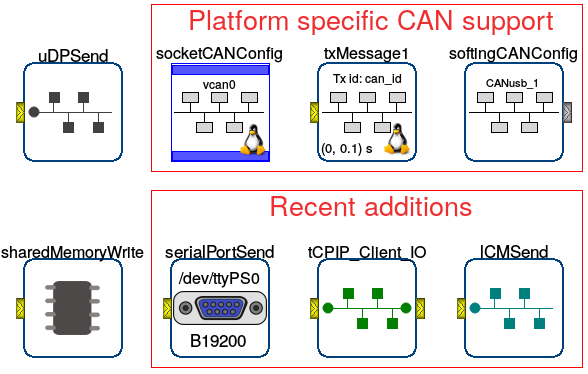
\includegraphics[width=0.9\columnwidth]{figures/OverviewCommunicationDevices}
  \caption{Supported communication devices from the \modelica{Blocks} package.}
  \label{fig:OverviewCommunicationDevices}
\end{figure}


Figure~\ref{fig:OverviewCommunicationDevices} gives an overview over the
supported devices. Cross-platform support for UDP and shared memory was already
available in the first released version of MDD. Support for serial port communication is
available since MDD v1.3 (Linux) and v1.4.0 (Windows). A client block for TCP/IP
socket communication was added in v1.4.0 (Windows) and v1.5.0 (Linux).
Furthermore, support for sending and receiving of Lightweight Communications and
Marshalling (LCM) datagrams\footnote{LCM project,
\url{https://lcm-proj.github.io/}} was added in v1.5.0.
LCM is a set of libraries and tools for message passing and data marshalling,
which is particularly targeted at low-latency real-time applications for
robotic systems \citep{Huang2010}.

Basic support for the Controller Area Network bus (CAN bus) is available by two
different block sets. The first is based on the CAN Layer2 API from
Softing\footnote{Softing, http://industrial.softing.com/} and restricted to the
Windows platform. The second uses the SocketCAN
interface provided by the Linux kernel.

\paragraph{Packaging Concept}

Communication devices like UDP or shared memory use a common packaging concept
in order to send or receive data. Therefore, the same packager can be used with
different communication devices. Figure~\ref{fig:PackagingConcept} shows an
example in which a package consisting of three variables of type \modelica{Real}
followed by a variable of type \modelica{Integer} is either transmitted using
shared memory or UDP blocks. Switching between the two communication devices
is achieved by simply replacing the corresponding device block.
\begin{figure}[htb]
  \centering
  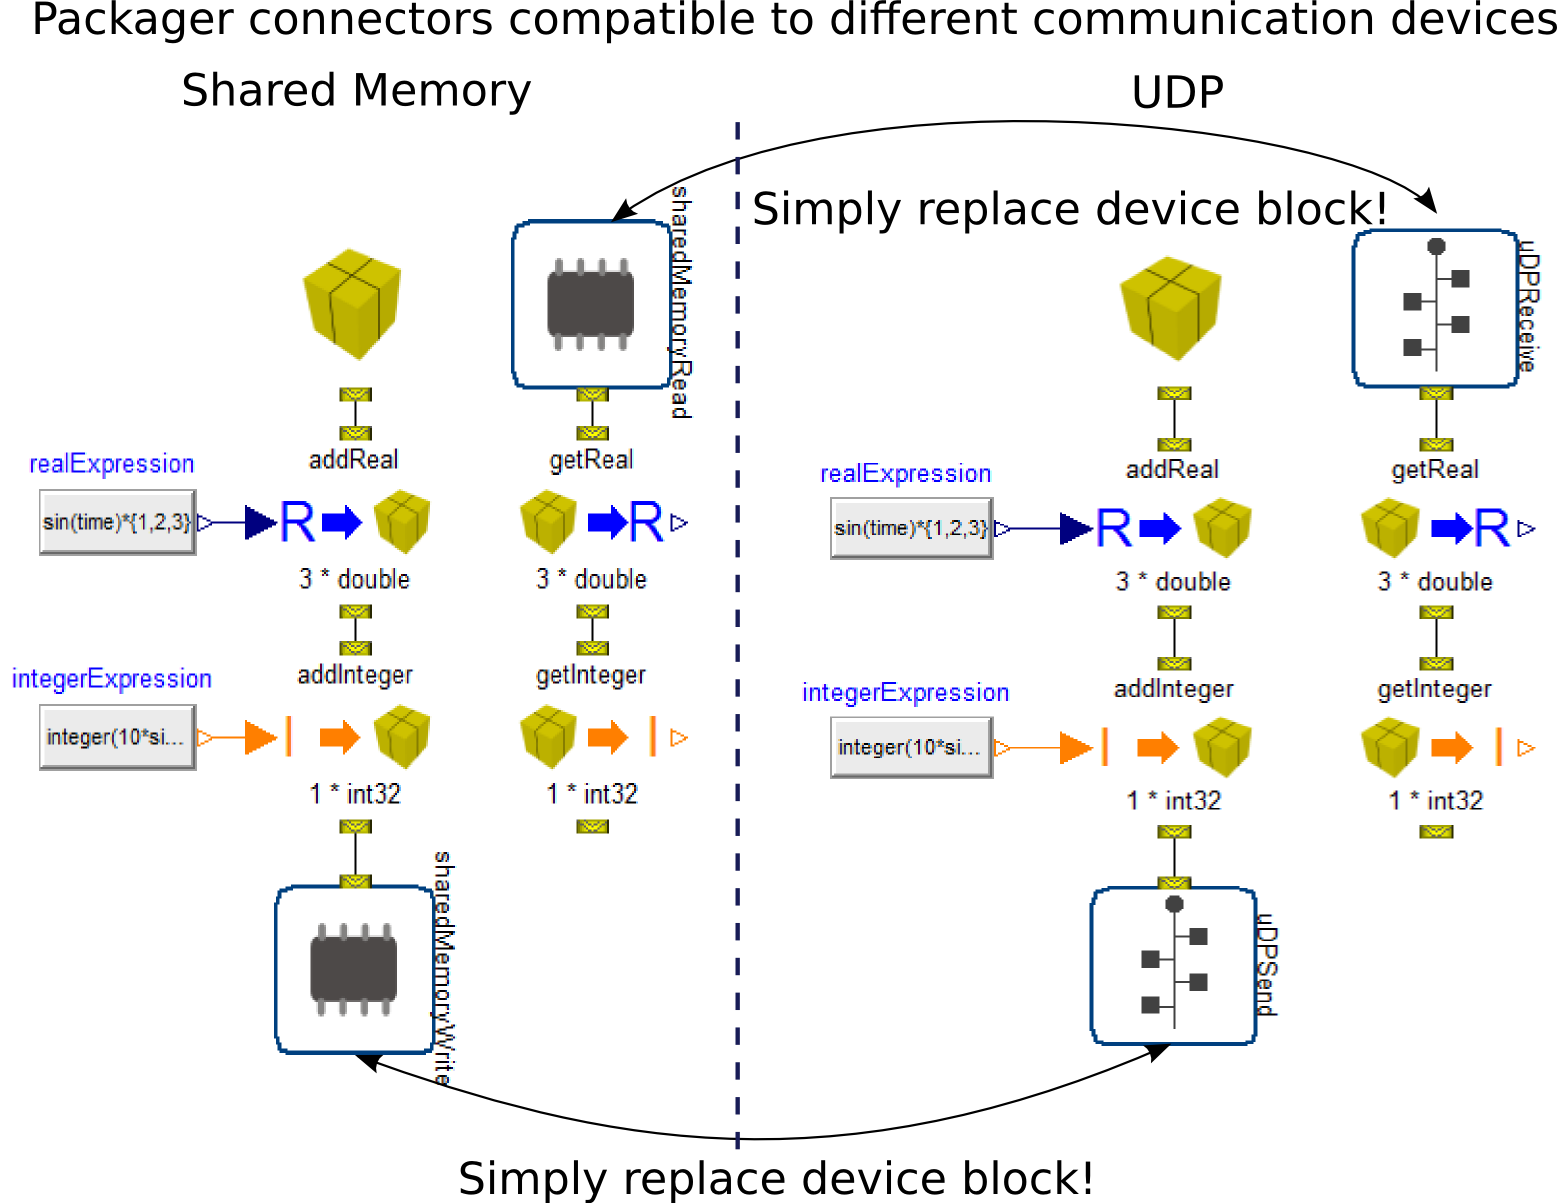
\includegraphics[width=1.0\columnwidth]{figures/PackagingConcept}
  \caption{Simple switching of communication devices due to common packaging concept
  in order to send or receive data.}
  \label{fig:PackagingConcept}
\end{figure}

The packages are constructed by using blocks from the \modelica{Packaging}
sub package (see Figure~\ref{fig:MDDPackageBrowseScreenshot}). In the initial
design of MDD it was expected that different packaging concepts would be
supported which share a common connector interface. However, As of MDD v1.5.0
the \modelica{SerialPackager} is the only available packager. It allows
to periodically add (or retrieve) fixed size vectors to (or from) a package.
Figure~\ref{fig:SerialPackagerBlocks} shows the available blocks for serializing
Modelica variables into a ``package''.
\begin{figure}[htb]
  \centering
  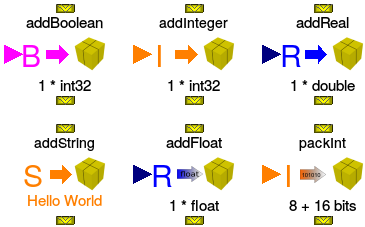
\includegraphics[width=0.6\columnwidth]{figures/SerialPackagerBlocks}
  \caption{\modelica{SerialPackager} blocks for adding variables to a package.}
  \label{fig:SerialPackagerBlocks}
\end{figure}

At the C side, a package is a C byte array in which C variables with
respectively indicated type are simply successively appended in a data-flow
prescribed order. For example, in Figure~\ref{fig:PackagingConcept} the
resulting byte array starts with three double values ($3 \times 8$ bytes)
followed by one int32 value ($4$ bytes), resulting in a byte array of size 28.
For the sake of providing an illustrative example at the C language level
the following C code snippet constructs a structurally equal package named
\clang{data} (the example shall shed light on the concept, it does not
advocate a coding style using magic numbers):
\begin{lstlisting}[language=C]
double v1[3] = {1.1, 2.2, 3.3};
int v2 = 4;
unsigned char* data = (unsigned char*) calloc(28, sizeof(unsigned char));
memcpy(&data[0], &v1[0], sizeof(v1));
memcpy(&data[24], &v2, sizeof(v2));
\end{lstlisting}

Figure~\ref{fig:SerialPackagerBlocks} shows the blocks for adding
variables to a package, symmetrically, blocks are available for retrieving variables from a
package. Using these blocks is deemed to be rather
intuitive with the notable exception of the \modelica{packInt} block. This
block allows to pack unsigned integer values at the bit level. The number of
bits used for encoding is set by a parameter \modelica{width}, therefore the maximum value
of the integer signal that can be encoded is $2^{\mathrm{width}} - 1$. A
parameter \modelica{bitOffset} allows to specify the bit at which the encoding starts
relative to the preceding block. Since MDD v1.3 most blocks support specifying
the byte ordering (big-endian or little-endian format).

It is simple to use the
\modelica{SerialPackager} blocks for deserializing data which has been serialized by it
(see Figure~\ref{fig:PackagingConcept}). In practice, however, communication
typically needs to be established with a remote station which is unrelated to
the Modelica model. As long as this remote station periodically sends or
receives structurally static, fixed sized packages it is usually quite
convenient to establish a communication using the MDD blocks. If the remote
station uses a more dynamic protocol it becomes more difficult. In some cases
using the \textsf{Function Layer} directly (instead of the \textsf{Block Layer})
can provide additional flexibility for coping with more dynamic protocols.
However, the main use-case for the \modelica{SerialPackager} concept is periodically
sent, structurally static data. This restrictions may be relieved in
future versions of MDD by providing additional ``Packagers'' that support more
flexible means of packaging data.

It turned out that the \modelica{SerialPackager} blocks were a major hurdle for
extending the number of Modelica tools which support MDD. They use a rather
intricate mechanism for propagating a ``package'' between connected blocks
which is discussed further in Section~\ref{sec:ModelicaStandardCompliance}.

\subsubsection{Hardware I/O}

Package \modelica{HardwareIO} (see
Figure~\ref{fig:MDDPackageBrowseScreenshot}) is intended for data acquisition
hardware like digital-analog converter (DAC), analog-digital converter (ADC) and
other interface hardware.

\begin{figure}[htb]
  \centering
  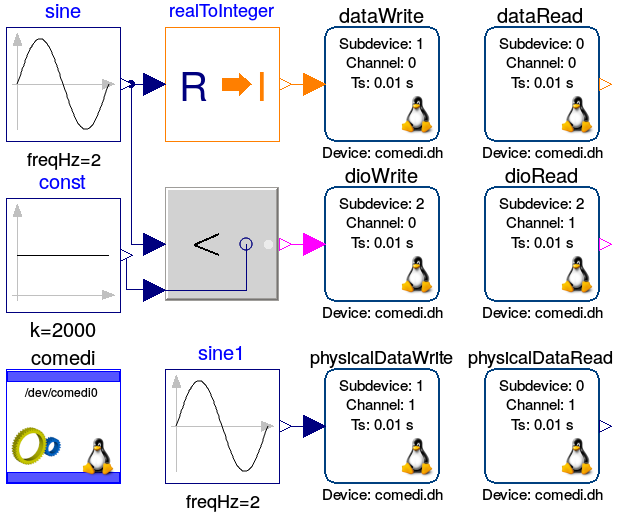
\includegraphics[width=0.9\columnwidth]{figures/MDDComedi}
  \caption{Accessing data acquisition hardware via the Linux
  control and measurement device interface ``Comedi''.}
  \label{fig:MDDComedi}
\end{figure}

As of MDD v1.5.0 it contains only one sub package which
provides support for the Linux control and measurement device interface
``Comedi''. The Comedi project develops open-source drivers, tools, and
libraries for data acquisition\footnote{Comedi project,
\url{http://www.comedi.org/}}. The project provides a common interface for
accessing supported data acquisition hardware (see the website for supported
hardware). The MDD library provides an interface to the Comedi user-space
library.

Figure~\ref{fig:MDDComedi} shows an example model which uses the provided
blocks. Configuration of the device is performed in the Modelica record named
\modelica{comedi}. The record contains an external object \modelica{dh} of type
\modelica{ComediConfig} which contains the Comedi device handle and is passed in
as a parameter to the other blocks (\modelica{comedi.dh}). Using external
objects in records is not standard compliant to Modelica v3.3 \citep{ModelicaAssociation2012} which is
further discussed in Section~\ref{sec:ModelicaStandardCompliance}.

Writing or reading raw integer values to DAC or from ADC channels is provided by
blocks \modelica{DataWrite} or \modelica{DataRead}, respectively. These blocks have
each a variant which works with physical values, instead of the raw integer
values  (\modelica{PhysicalDataWrite} and \modelica{PhysicalDataRead}).
Blocks \modelica{DIOWrite} and \modelica{DIORead} support digital input and
output (DIO) channels.


\vspace{0.5cm}
\BTHI{Write something about ``EmbeddedTarges'' features, here or write in in
``Applications and link to it?

TODO: Add a link to the project website somewhere!

Possibly cover new features in more detail if
enough time and paper space. New features:
\begin{itemize}
  \item Big endian
  \item Serial port on Win
  \item TCP/IP client
  \item LCM / UDP Broadcast
  \item Bluetooth
  \item MQTT
  \item \ldots
\end{itemize}
}


%%% \BTHI{Snippets that I want possibly reuse for the standard compliance}
% discussion The definition of the \modelica{SerialPackager} input connector is given below.
% \begin{lstlisting}[language=modelica]
% connector PackageIn "Packager input connector"
%   input Modelica_DeviceDrivers.Packaging.
%     SerialPackager pkg;
%   input Boolean trigger;
%   input Real dummy;
%
%   output Boolean backwardTrigger;
%   output Integer userPkgBitSize;
%   output Integer autoPkgBitSize;
% end PackageIn;
% \end{lstlisting}
% Most notably connector \modelica{PackageIn} contains an element
% \modelica{pkg} which is an external object of type \modelica{SerialPackager}.
%
% It would be
% possible to replace the Modelica configuration record by a configuration
% block, though \ldots

\section{Modelica Standard Compliance}
\label{sec:ModelicaStandardCompliance}
\BTHI{TODO: Thomas, Bernhard}

\subsection{Enhancements}

\subsection{Pitfalls and Open Issues}


Aide-mémoire:
\begin{itemize}
  \item Serialpackager
  \item Automatic buffer size
  \item External objects in equation
  \item Construction of external objects in record
  \item Linking to platform-dependent system libraries
  \item Missing fixed attribute for String
  \item Support of several include directories
\end{itemize}

\section{Applications}
\label{sec:Applications}

\subsection{Arduino}
\BTHI{TODO: Volker}

The Arduino\footnote{Arduino, \url{https://www.Arduino.cc}} is an open-source electronics platform which makes it very easy to read sensors, process the data and send it to another device via a serial connection.
With the help of the \emph{Modelica\_DeviceDrivers} serial port implementation, the Arduino can be utilized to make sensor data available in a real-time Modelica model, as depicted in Figure \ref{fig:arduino}.
With the help of potentiometers or other deflection sensors, customized control devices can be built.

As an exemplary application, self-built pedals for a driving simulator can be equipped with a sensor in order to measure the displacement. The pedal itself is a steel sheet, mounted on a revolute joint and a shock spring.
The measured deflection is transferred via a serial connection to a \textit{Blocks.Communication.SerialPortReceive} in order to drive a virtual vehicle.
Therefore, expensive or unavailable input devices can be substituted by self-built constructions.


\begin{figure}[htb]
	\centering
	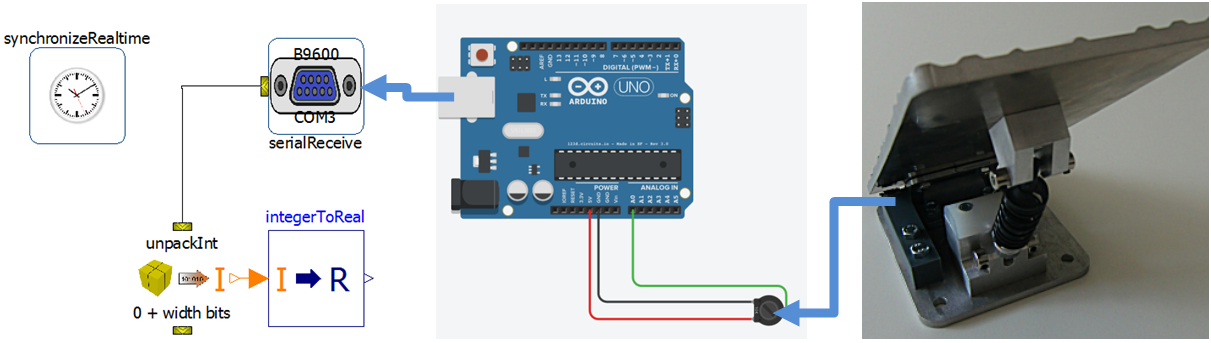
\includegraphics[width=0.9\columnwidth]{figures/arduino}
	\caption{Setup to read potentiometer deflection during realtime simulation with MDD serial port model.}
	\label{fig:arduino}
\end{figure}

By using a Bluetooth module with \textit{Serial Port Profile, SPP} a wireless connection between Arduino is handled in the same way as a physical USB-connection. No further modifications are necessary to implement a wireless control device.

\subsection{Arduino, Raspberry PI, embedded control}
\label{sec:EmbeddedControl}
\BTHI{TODO: Bernhard, Martin}

\subsection{HID Joystick}
\BTHI{TODO: Volker }

\subsection{DLR Demonstrators}
\BTHI{Tobias}

At the DLR Institute of System Dynamics and Control, several simulator systems
utilize the \emph{Modelica\_DeviceDrivers} library for inter-system
communication and querying of input devices.

\begin{figure}[htb]
  \centering
  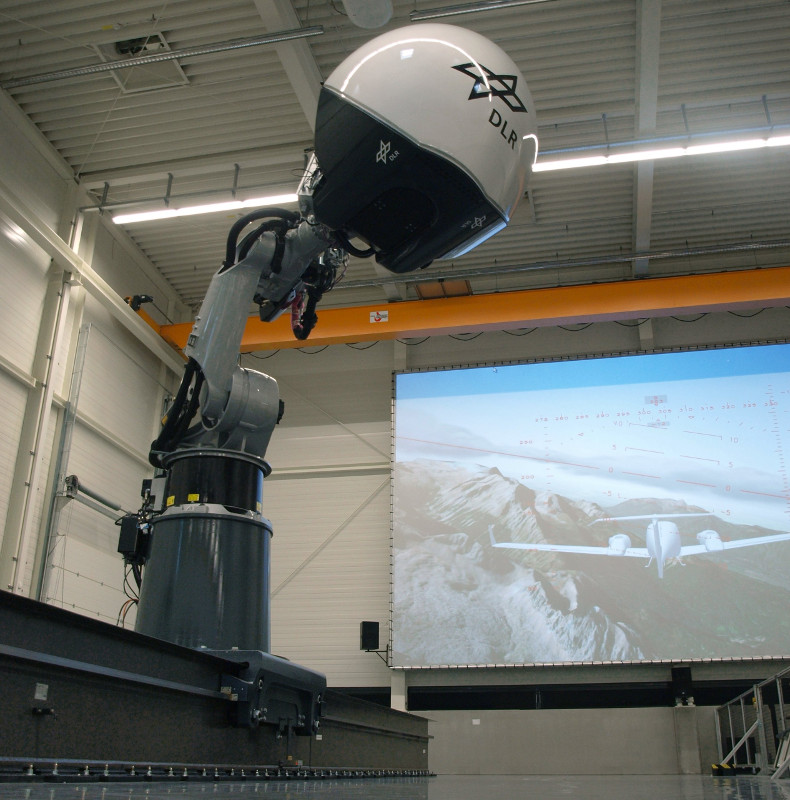
\includegraphics[width=0.9\columnwidth]{figures/DLRRoboticMotionSimulator}
  \caption{The DLR Robotic Motion Simulator.}
  \label{fig:DLRRoboticMotionSimulator}
\end{figure}
The DLR Robotic Motion Simulator \citep{bellmann2011dlr} is a 7 axis driving and
flight simulator based on an industrial robot arm (see
Figure~\ref{fig:DLRRoboticMotionSimulator}). The main use of this motion
simulator is the evaluation of input devices such as side-sticks, steering
wheels, pedals, etc., as well as the test and validation of control algorithms
in terms of stability and real-time capability. The control architecture of the
simulator uses blocks from the MDD library in several ways:
\begin{itemize}
  \item Input devices such as force-feedback steering wheels are connected via CAN Bus
and integrated in the software framework via the CAN blocks of the library, the same
applies for a force-feedback side-stick.
  \item Other, consumer based input devices such as pedals or Airbus styled flight
controls are connected via the \modelica{JoystickInput} block of the library.
  \item The control architecture for the robot consists of two Modelica simulations on
two different computers: First, the real-time path-planning running on a
real-time Linux system controlling the movements of the robot, and second, the
control panel running on a standard Windows system. The control panel is used to
change parameters such as washout filter modes (the washout filter maps the
movement of road vehicles / airplanes to the workspace of the simulator) and
gives an overview on the actual robot's position and telemetry. All real-time critical
communication (\textit{e.g.}, the simulated road vehicle / airplane forces and
angular velocities inputs for the real-time path-planning, or the control panel
inputs/outputs) are communicated via the library's UDP blocks and the serial
packaging system.
\end{itemize}

\begin{figure}[htb]
  \centering 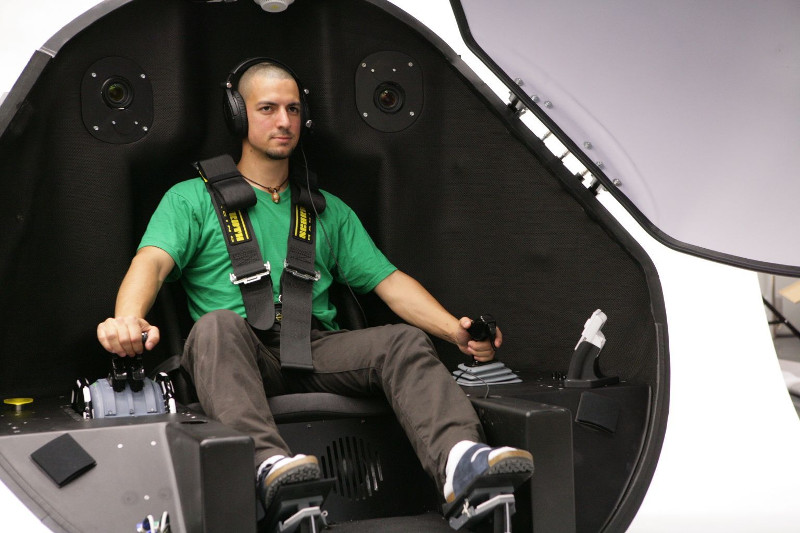
\includegraphics[width=0.9\columnwidth]{figures/DLRSimulatorCabin}
  \caption{View into the simulator cabin of the DLR motion simulator. The
  instrumentation package is replaceable, so that the simulator cabin can be
  easily adapted for different simulation types, \textit{e.g.}, for driving or
  flight simulation.}
  \label{fig:DLRSimulatorCabin}
\end{figure}
Figure~\ref{fig:DLRSimulatorCabin} shows the inside of the simulator cabin.
The instrumentation package can be adapted
for different simulation types or for testing different input concepts.
An on-board computer is used to query input devices, to display information on
control screens, and to project the pilot's outside view visualization on the
embracing concave dome shell. These
tasks are performed using Modelica models, where the
\modelica{SynchronizeRealtime} block is used for real-time
synchronization. Also, communication with the other simulation components is
performed partly via the UDP blocks.

\begin{figure}[htb]
  \centering
  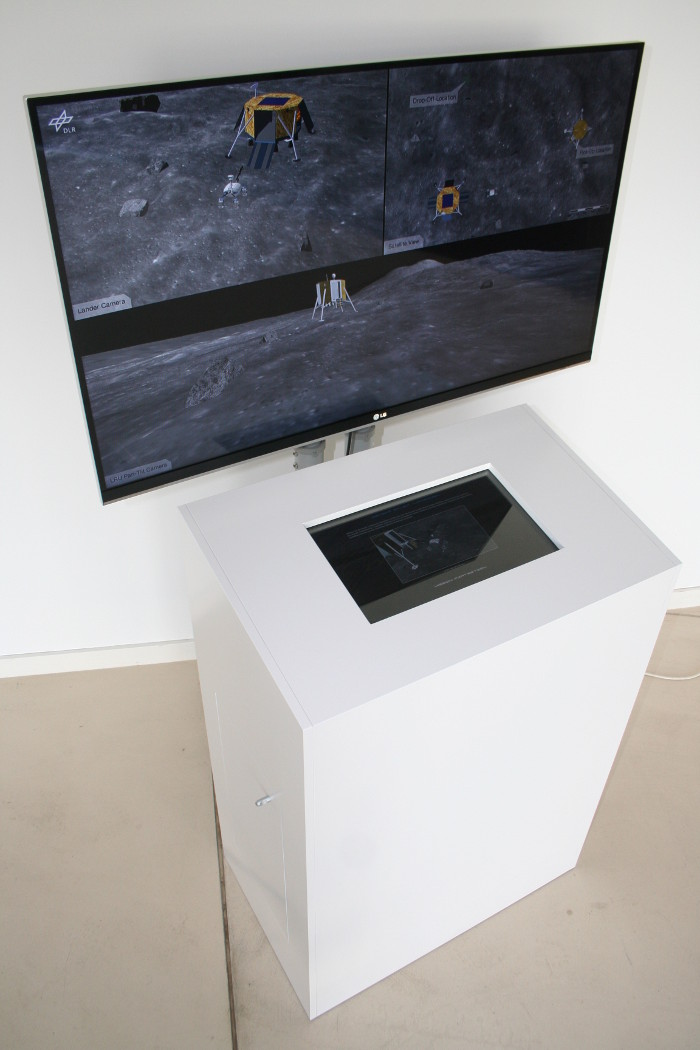
\includegraphics[width=0.5\columnwidth]{figures/DLRROBEX}
  \caption{DLR ROBEX technology demonstrator.}
  \label{fig:DLRROBEX}
\end{figure}
Figure~\ref{fig:DLRROBEX} shows the ROBEX demonstrator, another system which
utilizes the MDD library which was developed as a technology demonstrator
for a science exhibition. This demonstrator allows the user to command a rover
on a scientific lunar mission. The missions goal is to pick up a sensor package from a nearby
lander and to place it on a marked position on the lunar surface. The user
controls the rover via an android app which is running on a tablet in front of
the simulator screen. On the screen, the visualization of the rover is displayed.
The underlying Modelica simulation performs the multi-body simulation of the
rover and utilizes the DLR Visualization library to display the rover and the
scenery. It uses MDD blocks to communicate with the tablet and the
\modelica{SynchronizeRealtime} block to adjust the simulation speed.

In very similar ways, the library is also used in several other simulator and
demonstrator systems, \textit{e.g.}, a drilling rig training simulator, several
desktop flight simulators, or a rover software-in-the-loop development
environment.

\section{Outlook}
\BTHI{TODO: Bernhard, Thomas, Volker}

\section*{Acknowledgements}


%%% choose one of the following: %%%
%% References using bibtex (default)
\bibliography{modelica2017_Modelica_DeviceDrivers}

%% References using biber and biblatex
%\printbibliography

\end{document}
